\documentclass[tikz,border=8pt]{standalone}
% Shared look for every TikZ diagram. Load with \input{../../tools/tikz-style.tex}
\usepackage[T1]{fontenc}
\usepackage{lmodern}
\renewcommand{\sfdefault}{lmr}  % diagrams use the same serif as the text
\usetikzlibrary{arrows.meta, positioning, shapes.geometric, calc, fit, backgrounds}
\definecolor{cblue}{HTML}{4C78A8}
\definecolor{corange}{HTML}{F58518}
\definecolor{cgreen}{HTML}{54A24B}
\definecolor{cred}{HTML}{E45756}
\definecolor{cpurple}{HTML}{B279A2}
\definecolor{cgrey}{HTML}{6B6B6B}
\tikzset{
  every picture/.style={font=\sffamily, line width=1.2pt},
  box/.style={draw=#1, fill=#1!12, rounded corners=4pt, align=center, inner sep=7pt, minimum height=1.1cm},
  box/.default=cgrey,
  arrow/.style={-{Stealth[length=3mm]}, draw=cgrey, line width=1.4pt},
  title/.style={font=\sffamily\bfseries\Large},
  note/.style={font=\sffamily\small, text=cgrey, align=center},
}
\AtBeginDocument{\hyphenpenalty=10000 \exhyphenpenalty=10000}

\begin{document}
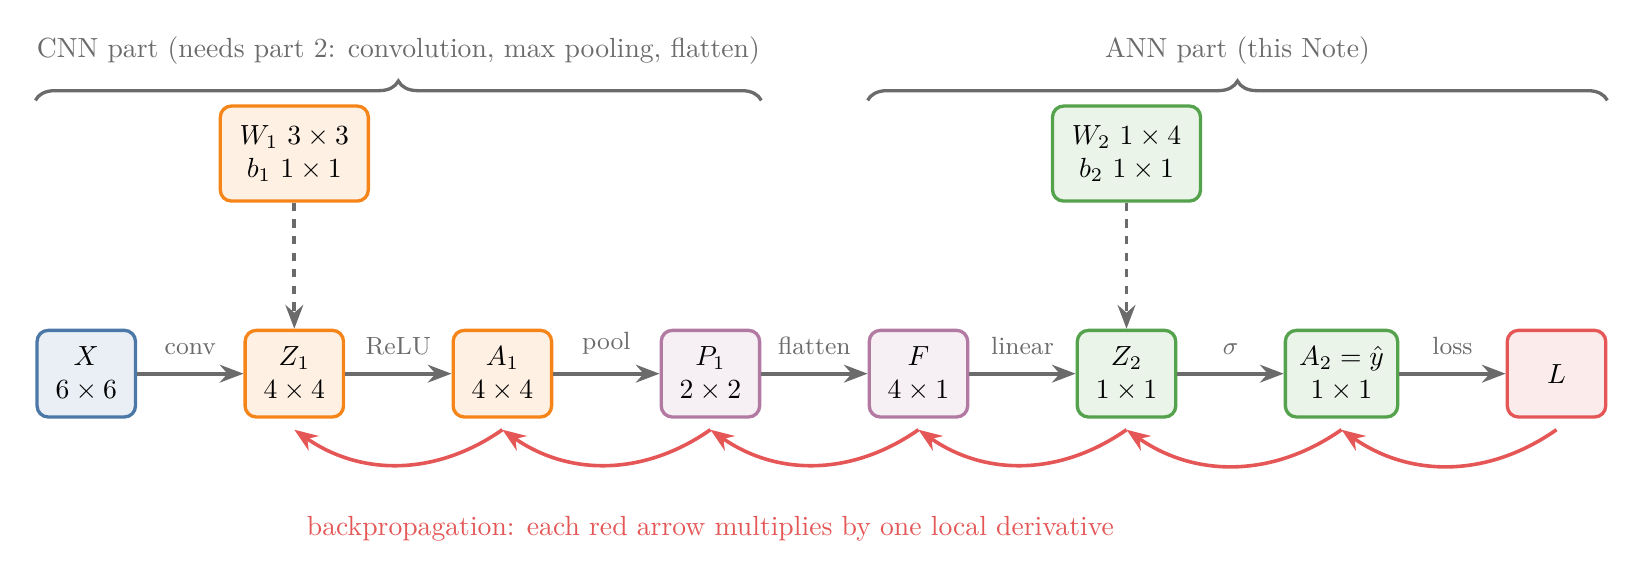
\begin{tikzpicture}[node distance=1.35cm, every node/.append style={font=\sffamily}]
  \tikzset{v/.style={box=#1, minimum width=1.25cm, inner sep=5pt}}
  \node[v=cblue] (x) {$X$\\$6 \times 6$};
  \node[v=corange, right=of x] (z1) {$Z_1$\\$4 \times 4$};
  \node[v=corange, right=of z1] (a1) {$A_1$\\$4 \times 4$};
  \node[v=cpurple, right=of a1] (p1) {$P_1$\\$2 \times 2$};
  \node[v=cpurple, right=of p1] (f) {$F$\\$4 \times 1$};
  \node[v=cgreen, right=of f] (z2) {$Z_2$\\$1 \times 1$};
  \node[v=cgreen, right=of z2] (a2) {$A_2 = \hat{y}$\\$1 \times 1$};
  \node[v=cred, right=of a2] (l) {$L$};
  \foreach \a/\b/\t in {x/z1/conv, z1/a1/ReLU, a1/p1/pool, p1/f/flatten, f/z2/linear, z2/a2/$\sigma$, a2/l/loss}{
    \draw[arrow] (\a) -- (\b) node[midway, above=3pt, font=\sffamily\small, text=cgrey, align=center] {\t};
  }
  \node[box=corange, above=1.6cm of z1, minimum width=1.2cm] (w1) {$W_1$ $3 \times 3$\\$b_1$ $1 \times 1$};
  \node[box=cgreen, above=1.6cm of z2, minimum width=1.2cm] (w2) {$W_2$ $1 \times 4$\\$b_2$ $1 \times 1$};
  \draw[arrow, dashed] (w1) -- (z1);
  \draw[arrow, dashed] (w2) -- (z2);
  % backward
  \foreach \a/\b in {l/a2, a2/z2, z2/f, f/p1, p1/a1, a1/z1}{
    \draw[-{Stealth[length=3mm]}, draw=cred, line width=1.3pt] ([yshift=-4pt]\a.south) to[bend left=35] ([yshift=-4pt]\b.south);
  }
  \node[text=cred, below=1.1cm of p1, align=center] (lbl) {backpropagation: each red arrow multiplies by one local derivative};
  \draw[decorate, decoration={brace, amplitude=7pt}, cgrey] ([yshift=2.9cm]x.north west) -- ([yshift=2.9cm]p1.north east)
    node[midway, above=9pt, text=cgrey] {CNN part (needs part 2: convolution, max pooling, flatten)};
  \draw[decorate, decoration={brace, amplitude=7pt}, cgrey] ([yshift=2.9cm]f.north west) -- ([yshift=2.9cm]l.north east)
    node[midway, above=9pt, text=cgrey] {ANN part (this Note)};
\end{tikzpicture}
\end{document}
